\documentclass[11pt]{article}
\usepackage{amsmath, amsfonts, amsthm, amssymb}  % Some math symbols
\usepackage{mathtools} % defines \coloneqq
\usepackage{enumerate}
\usepackage{fullpage}
\usepackage{graphics}

\title{CMU Seats Project Proposal}
\author{Raaid Tanveer}
\date{\today}

\begin{document}
  \maketitle
  \section{Overview}
  CMU Seats will be a seat-finding application that Carnegie Mellon University students can use for finding an empty seat on campus. Moreover, this application will allow students to find seats that are close to their friends, and for seated individuals to signal empty seats nearby to their friends. 

  \section{Use Cases}
  The application will cater to primarily two groups of users:
  \begin{enumerate}[(a)]
    \item \textbf{Seat Finders}: These are the individuals who will be looking for a seat on campus. They will use the application for:
    \begin{itemize}
      \item Finding seats that are in a given region or building
      \item Finding a seat closest to them
      \item Finding a seat close to their friends
      \item Signaling that a seat that has been suggested by the application is occupied, and finding a new seat afterwards
    \end{itemize}
    \item \textbf{Seat Occupiers}: These are the individuals who have a seat. They will use the application for:
    \begin{itemize}
      \item Signaling the number of empty seats around them
      \item Signaling to particular individuals that they have seating available around them
    \end{itemize}
  \end{enumerate}
  \newpage
  \section{System Design}
  \subsection{DB Schema}
  \begin{center}
    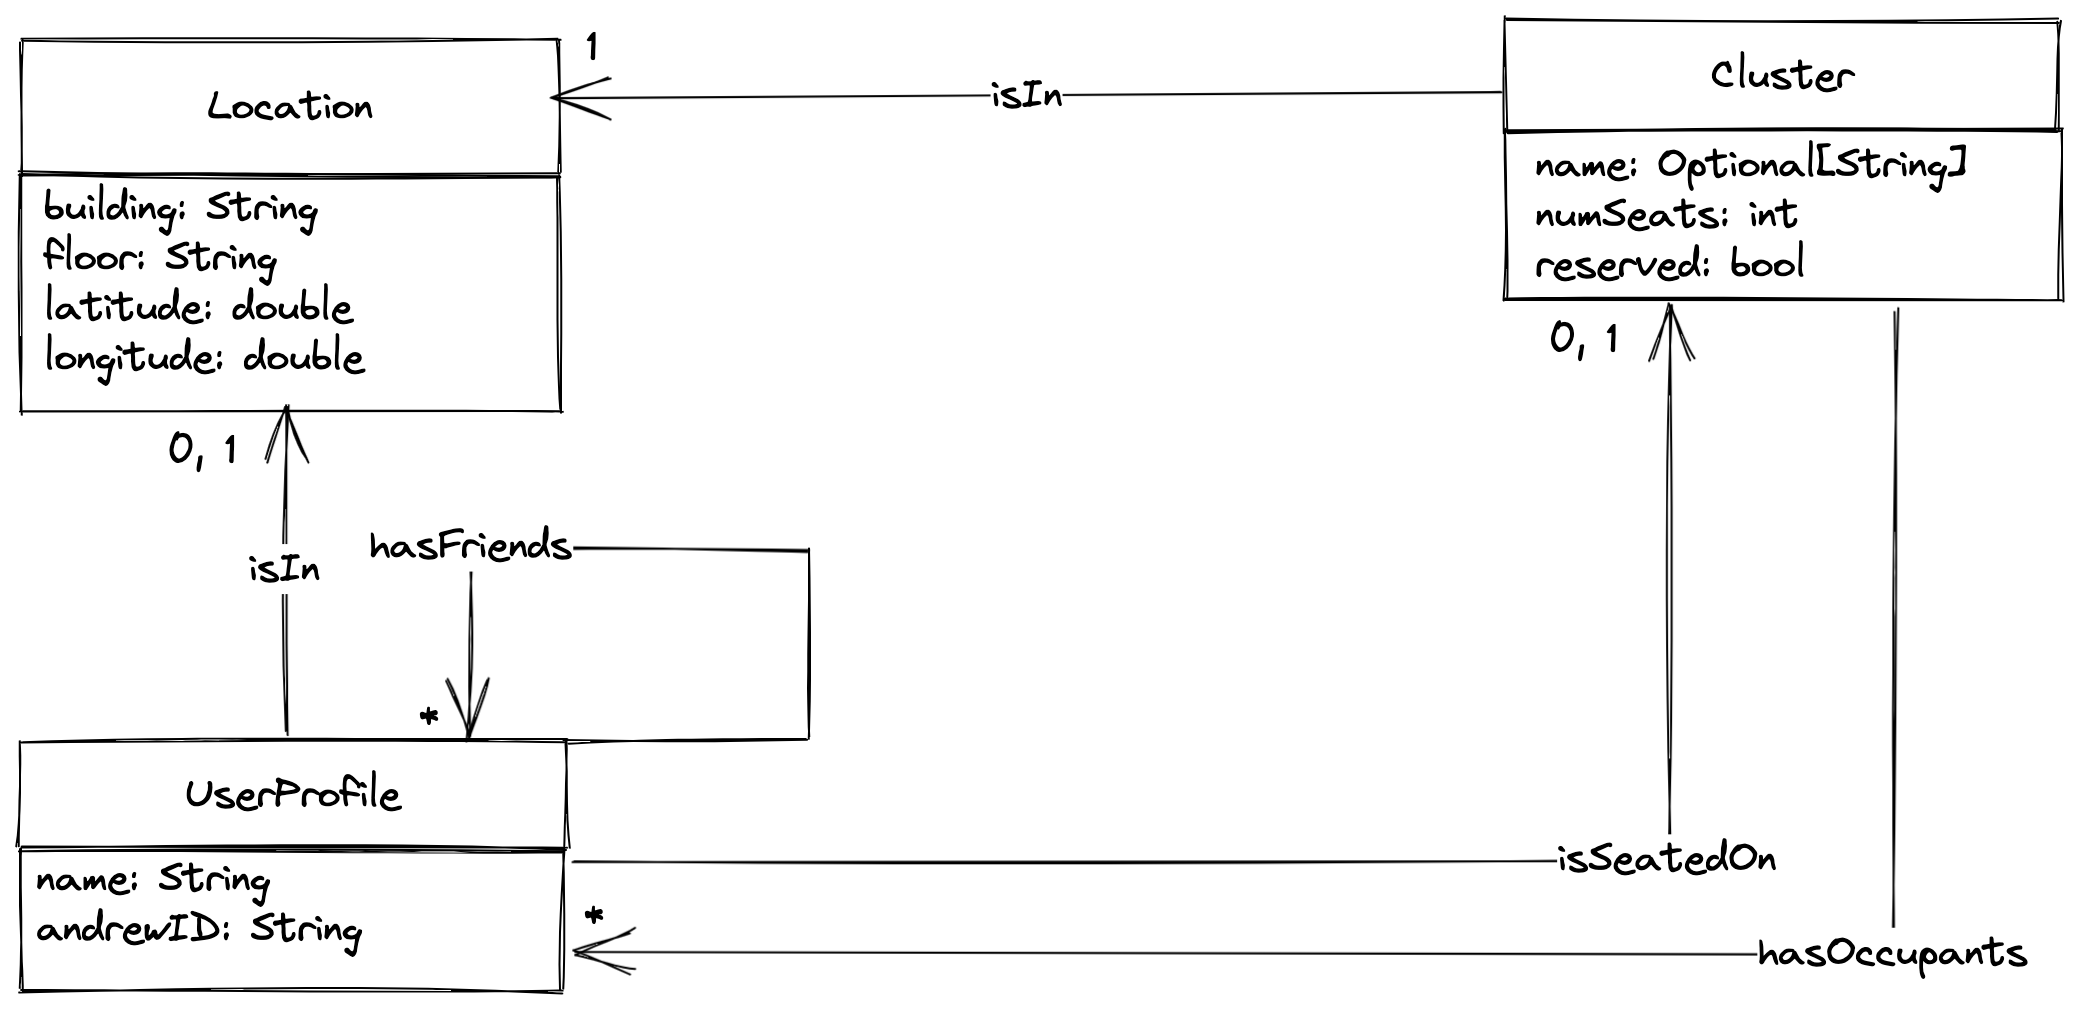
\includegraphics[scale=0.2]{CMUSeats DB Schema.png}
  \end{center}
  \textbf{Legend:} 
  \begin{itemize}
    \item The arrows indicates that the pointed to object is stored by the object that is pointed from, with the relationship labeled by the text in the arrow
    \item \(0, 1\) label on the pointed to object means an optional storage of the pointed to object by the object that is pointed from.
    \item \(1\) label on the pointed to object means exactly one of the pointed to object is stored by the pointed from object.
    \item \(*\) label on the pointed to object means zero or more of the pointed to object is stored by the pointed from object. 
  \end{itemize}
  \subsection{Key Functionality}
  \begin{enumerate}
    \item 
  \end{enumerate}
  \newpage
  \section{Performance Analyses}
  There's a few different cases that we want to analyze. 
  \subsection{No Users of the App}
  Let the topology of seats be represented as a \(d\)-regular graph on \(n\) vertices. Assume that users flow in at time \(t\) at a rate of \(X_t \sim \text{Poisson}(\lambda)\). Furthermore, assume that each user \(u\), if they obtain a seat, occupy that seat for \(S_u \sim \text{Poisson}(\nu)\) time. Lastly, assume that users spawn uniformly at random on vertices (which they initially cannot sit on) and travel with uniformly at randomly to it's neighbor, and sit there if that is free. Otherwise, they travel to another vertex from there uniformly at random. If two or more users end up wanting to sit at the same seat together, neither gets the seat and they retry. They retry for at most \(k\) tries. 
\end{document}
